\section{Le modèle de régression linéaire simple}
\label{sec:ModèleRLS}

Le modèle de régression linéaire simple est un modèle dans lequel on cherche à expliquer une variable endogène $Y$ en fonction d'une seule variable exogène $x$. Il s'exprime comme suit
\begin{eqnarray}
 Y_i = \beta_0 + \beta_1 x_i + \varepsilon_i, 
 \label{eq:reg_lin_simple}
\end{eqnarray}
où 
\begin{itemize}
    \item $Y_i$ est une variable aléatoire représentant la réponse de l'unité $i$;
    \item $x_i$ est la valeur (connue) de la variable explicative de l'unité $i$;
    \item $\beta_0$ est le paramètre associé à l'ordonnée à l'origine de la droite;
    \item $\beta_1$ est le paramètre associé à la pente de la droite;
    \item $\varepsilon_i$ est une variable aléatoire représentant le terme d'erreur de l'unité $i$.
\end{itemize}
Il est important de comprendre quelles quantités sont supposées constantes ou aléatoires dans le modèle \eqref{eq:reg_lin_simple}, à savoir
 \begin{itemize}
 \item $Y_1,\ldots, Y_n$ sont des variables aléatoires;
 \item $x_1,\ldots,x_n$ sont des valeurs considérées constantes;
 \item $\beta_0$ et $\beta_1$, les paramètres du modèle, sont constants;
 \item $\varepsilon_1,\ldots,\varepsilon_n$ sont des variables aléatoires.
  \end{itemize}
Les paramètres du modèle \eqref{eq:reg_lin_simple} sont inconnus et doivent être estimés. Pour les estimer, nous disposons de $n$ réalisations, soit les couples $(x_i, y_i)$, pour $i=1, \dots, n$. À noter que $y_i$ est la réalisation de la variable aléatoire $Y_i$, pour $i = 1, \dots, n$.


\subsection{Postulats du modèle de RLS}
\label{sec:Postulats}

Pour développer la théorie de la régression linéaire, il est nécessaire de formuler certains postulats sur le modèle défini en \eqref{eq:reg_lin_simple}. Ces postulats peuvent être énoncés mathématiquement en termes d'hypothèses sur les termes d'erreur $\varepsilon_i$ du modèle:
\begin{enumerate}
  \item[$\mathcal{P}_1$.] La linéarité de la relation entre la variable réponse et la variable explicative:
  
  $\esp[\varepsilon_i]=0 \mbox{ pour } 1\leq i \leq n$.
 \item[$\mathcal{P}_2$.] L'homoscédasticité (variance constante) des observations de la variable réponse:

 $\var[\varepsilon_i]=\sigma^2 \mbox{ pour } 1\leq i \leq n$.
 \item[$\mathcal{P}_3$.] L'indépendance des observations de la variable réponse:

 $\cov(\varepsilon_i,\varepsilon_j)=0 \mbox{ pour } i \neq j.$
 \item[$\mathcal{P}_4$.] La normalité des termes d'erreur:
  
  $\varepsilon_1, \cdots , \varepsilon_n \sim \N(0,\sigma^2)$.
\end{enumerate}
Le premier postulat est nécessaire pour l'interprétation des paramètres du modèle, et indique simplement que le modèle linéaire est approprié pour modéliser la relation entre les variables d'intérêt. Les deux postulats suivants permettent d'estimer la variance des estimateurs de $\beta_0$ et $\beta_1$. Obtenir une telle mesure de précision des estimateurs ponctuels est très important en pratique.
À ces trois postulats, on doit souvent ajouter le quatrième postulat sur l'hypothèse de normalité des termes d'erreur. Il s'agit d'un postulat plus fort généralement utilisé parce qu'il permet de construire des intervalles de confiance et de faire des tests d'hypothèses aisément\footnote{Il est également possible d'obtenir des intervalles de confiance et des tests d'hypothèses sans poser le postulat de normalité des erreurs, en utilisant par exemple la méthode du bootstrap.}. On verra également que ce postulat est nécessaire à la mise en {\oe}uvre de la méthode du maximum de vraisemblance pour l'estimation des paramètres.

Il est évidemment possible que ces 4 postulats ne soient pas vérifiés en pratique. Nous verrons dans ce cours comment tester si chacun des postulats est vérifié et comment modifier le modèle au besoin. Nous verrons aussi brièvement d'autres modèles de régression qui peuvent être utilisés si une ou plusieurs des conditions d'application de la RLS ne sont pas vérifiées.


\subsection{Interprétation de $\beta_0$ et $\beta_1$}
\label{sec:Interprétation}


La \autoref{fig:rls} illustre le modèle de régression linéaire simple. La ligne droite représente la valeur moyenne de $Y$ en fonction de la valeur de $x$. Les variables $Y_i$ sont distribuées de façon aléatoire autour de cette droite. Les termes d'erreur sont les différences entre les $Y_i$ et la droite. Comme la variance de ces termes est constante en $x$, la distance moyenne des points à la droite est la même pour toute valeur de $x$. Finalement, l'absence de corrélation entre les termes d'erreur
signifie que la valeur d'un terme d'erreur n'est pas influencée par la valeur des autres termes d'erreur.

\begin{figure}[h!]
\centering
\begin{tikzpicture}[scale=1]
%------------------------------------------------
% Axes
\draw[-{Latex[length=8pt]}] (0,0) -- (0,7.5);
\node at (-0.3,7.3) {$y$};
\draw[-{Latex[length=8pt]}] (0,0) -- (7.8,0);
\node at (7.6,-0.3) {$x$};
%------------------------------------------------
% Droite de régression
% y = beta_0 + beta_1 x
\draw[thick] (-0.7,0.2) -- (7.2,7.2);
%------------------------------------------------
% Ordonnée à l'origine beta_0
\draw (-0.2,0.82) -- (0.3,0.82);
\node[left] at (-0.2,0.82) {$\beta_0$};
%------------------------------------------------
% Observations
\fill
    (1.3,2.6) circle (0.09)
    (1.7,1.8) circle (0.09)
    (2.1,2.1) circle (0.09)
    (2.5,2.8) circle (0.09)
    (2.9,3.0) circle (0.09)
    (3.3,3.5) circle (0.09)
    (4.5,4.2) circle (0.09)
    (3.3,4.5) circle (0.09);
%------------------------------------------------
% Première observation : x_1, y_1 et epsilon_1
% verticale x_1
\draw (3.8,-0.1) -- (3.8,4.2);
% horizontale vers Y_1
\draw (-0.1,3.0) -- (3.8,3.0);
% erreur epsilon_1
\node[right] at (3.8,3.4) {$\varepsilon_1$};
% point associé
\fill (3.8,3.0) circle (0.09);
% étiquette x_1
\node[below] at (3.8,-0.1) {$x_1$};
% étiquette Y_1
\node[left] at (0,3.0) {$Y_1$};
%------------------------------------------------
% Deuxième observation : x_2, y_2 et epsilon_2
% verticale x_2
\draw (4.3,-0.1) -- (4.3,5.0);
% horizontale vers Y_2
\draw (-0.1,5.0) -- (4.3,5.0);
% erreur epsilon_2
\node[left] at (4.3,4.7) {$\varepsilon_2$};
% point associé
\fill (4.3,5.0) circle (0.09);
% étiquette x_2
\node[below] at (4.3,-0.1) {$x_2$};
% étiquette Y_2
\node[left] at (0,5.0) {$Y_2$};
%------------------------------------------------
% Illustration de beta_1
% point sur la droite
\coordinate (A) at (5.0,5.2);
\coordinate (B) at (6.5,5.2);
\coordinate (C) at (6.5,6.6);
% lignes pointillées
\draw[dashed] (A) -- (B);
\draw[dashed] (B) -- (C);
% beta_1
\node[right] at (6.5,6.0) {$\beta_1$};
\end{tikzpicture}
\caption[Illustration du modèle de régression linéaire simple]{Illustration du mod\`ele de r\'egression lin\'eaire simple. }
\label{fig:rls}
\end{figure}
On interprète $\beta_0$ comme la valeur moyenne de $Y$ lorsque $x$ vaut zéro et $\beta_1$ comme l'accroissement moyen de $Y$ lorsque $x$ augmente d'une unité. Si $\beta_0 = 0$, l'espérance de $Y$ est nulle lorsque $x$ vaut zéro, et le modèle ne comporte pas d'ordonnée à l'origine. Si $\beta_1 = 0$, l'espérance de $Y$ ne dépend pas de $x$, du moins pas de façon linéaire.


\subsection*{Modèle centré}

Il arrive que la valeur moyenne de $Y$ lorsque $x$ vaut zéro soit difficile ou inutile à interpréter. On peut alors utiliser une version centrée du modèle,
\begin{eqnarray*}
 Y_i &=& \beta_0 + \beta_1 x_i + \varepsilon_i \\
 &=& \beta_0^* + \beta_1 (x_i - \overline{x}) + \varepsilon_i \text{ (version centrée)}.
\end{eqnarray*}
Dans la version centrée du modèle, l'interprétation de $\beta_1$ est inchangée, mais $\beta_0^*$ s'interprète comme étant la valeur moyenne de $Y$ lorsque $x$ vaut $\overline{x}$. On remarque que $\beta_0^* = \beta_0 + \beta_1 \overline{x}$.


\section{Estimation des paramètres}
\label{sec:estimation}

Dans le modèle de régression linéaire simple, on doit estimer trois paramètres: $\beta_0$ et $\beta_1$, qui décrivent la droite de régression, ainsi que $\sigma^2$, la variance des termes d'erreur. Deux approches communes pour estimer les paramètres d'un modèle de régression sont la méthode des moindres carrés et celle du maximum de vraisemblance. Dans les sections suivantes, on explique comment estimer les paramètres de régression à l'aide de ces deux approches, et on démontre qu'elles sont équivalentes sous le postulat de normalité $\mathcal{P}_4$.

\subsection{Méthode des moindres carrés}

Tel que mentionné au \autoref{sec:intro}, on attribue généralement la méthode des moindres carrés au mathématicien français Adrien-Marie Legendre (1752-1833). Plusieurs autres mathématiciens de l'époque ont aussi publié des travaux sur le sujet, notamment Carl Friedrich Gauss (1777-1855) et Robert Adrain (1775-1843).

Soit $\widehat{Y}_i$ la prévision du modèle pour l'observation $i$. On appelle résidu la différence entre $Y_i$, la variable réponse, et cette prévision $\widehat{Y}_i$. On le dénote $\widehat{\varepsilon}_i$, puisque c'est une estimation du terme d'erreur $\varepsilon_i$.

Avec la méthode des moindres carrés, on cherche à choisir les estimateurs $\widehat\beta_0$ et $\widehat\beta_1$ de façon à minimiser la somme des carrés des erreurs. On veut donc minimiser la fonction 
\begin{eqnarray}
g(\beta_0,\beta_1) =  \sum_{i=1}^n \varepsilon_i^2  =  \sum_{i=1}^n \left\{Y_i- (\beta_0+\beta_1 x_i)\right\}^2.
    \label{eq:MoindresCarres}
\end{eqnarray}
Puisque la fonction \`a minimiser possède de bonnes propri\'et\'es
(entre autres lisse et convexe), elle peut être minimisée en la dérivant par rapport \`a ${\beta}_0$ et ${\beta}_1$, puis en posant ces d\'eriv\'ees \'egales \`a z\'ero. On doit donc résoudre le système d'équations \`a deux inconnues suivant:
\begin{eqnarray}
\left\{ \begin{array}{ccc}
\frac{\displaystyle\partial}{\displaystyle\partial{\beta}_0}
\sum\limits_{i=1}^n(Y_i-{\beta}_0-{\beta}_1 x_i)^2
&=&\label{eq1} 0, \\
\frac{\displaystyle\partial}{\displaystyle\partial{\beta}_1}
\sum\limits_{i=1}^n(Y_i-{\beta}_0-{\beta}_1 x_i)^2
&=&\label{eq2} 0.
\end{array}
\right.
\end{eqnarray}

\subsubsection*{Estimation de $\beta_0$}

On dérive d'abord par rapport à $\beta_0$:
\begin{eqnarray*}
 \frac{\partial}{\partial \beta_0} \left\{\sum_{i=1}^n (Y_i - \beta_0 - \beta_1 x_i)^2\right\} &=& \sum_{i=1}^n 2(Y_i - \beta_0 - \beta_1 x_i)(-1)\\
 &=& -2( n \overline{Y} - n \beta_0 - n \beta_1 \overline{x}).
\end{eqnarray*}
On pose ensuite cette dérivée égale à zéro, et elle est évaluée au point $\left(\widehat\beta_0, \widehat\beta_1 \right)$. Il s'agit du point critique de la fonction $g(\beta_0,\,\beta_1)$:
\begin{eqnarray}
-2(n \overline{Y} - n \widehat\beta_0 - n \widehat\beta_1 \overline{x}) & = & 0, \nonumber\\
 \overline{Y} - \widehat\beta_0 - \widehat\beta_1 \overline{x} & = & 0, \nonumber\\
 \widehat\beta_0 & = &  \overline{Y} - \widehat\beta_1 \overline{x}.
\label{eq:beta0}
\end{eqnarray}

\begin{remarque}
 Il est à noter que l'équation \eqref{eq:beta0} signifie que la droite de régression passe nécessairement par le point de coordonnées $(\overline{x},\overline{Y})$:
\begin{eqnarray}
\overline{Y} = \widehat\beta_0+ \widehat\beta_1 \overline{x}.
 \label{eq:dbeta0egal0}
\end{eqnarray}
\end{remarque}

\subsubsection*{Estimation de $\beta_1$}

On dérive ensuite par rapport à $\beta_1$:
\begin{eqnarray*}
 \frac{\partial}{\partial \beta_1} \left\{\sum_{i=1}^n (Y_i - \beta_0 - \beta_1 x_i)^2\right\} &=& \sum_{i=1}^n 2(Y_i - \beta_0 - \beta_1 x_i)(-x_i)\\
 &=& -2 \left(\sum_{i=1}^n x_i Y_i - \sum_{i=1}^n  \beta_0 x_i - \sum_{i=1}^n  \beta_1 x_i^2 \right).
\end{eqnarray*}
En posant cette dérivée égale à zéro, en l'évaluant au point $\left(\widehat\beta_0, \widehat\beta_1 \right)$ et en utilisant  \eqref{eq:beta0}, on a
\begin{eqnarray*}
-2 \left( \sum_{i=1}^n x_i Y_i - \sum_{i=1}^n  \widehat\beta_0 x_i - \sum_{i=1}^n  \widehat\beta_1 x_i^2\right) & = & 0 \\
\sum_{i=1}^n x_i Y_i &= & \widehat\beta_0 \sum_{i=1}^n x_i + \widehat\beta_1 \sum_{i=1}^nx_i^2 \\
\sum_{i=1}^n x_i Y_i & = & (\overline{Y}-\widehat\beta_1 \overline{x}) \sum_{i=1}^n x_i + \widehat\beta_1 \sum_{i=1}^nx_i^2 \\
\sum_{i=1}^n x_i Y_i & = & \overline{Y} \sum_{i=1}^n x_i + \widehat\beta_1 \left(\sum_{i=1}^n x_i^2 - \overline{x}\sum_{i=1}^n x_i \right).
\end{eqnarray*}
On obtient l'estimateur 
\begin{equation}
\label{eq:beta1chapeau}
\widehat{\beta}_1 = \frac{\sum\limits_{i=1}^n x_i Y_i -\overline{Y} \sum\limits_{i=1}^n x_i}{\sum\limits_{i=1}^n x_i^2 - \overline{x}\sum\limits_{i=1}^n x_i}.
\end{equation}


Il est possible de réécrire $\widehat\beta_1$ sous les formes équivalentes suivantes:
\begin{equation*}
 \widehat{\beta}_1 =  \frac{\sum\limits_{i=1}^n x_i Y_i - n\overline{x}\overline{Y}}{\sum\limits_{i=1}^n x_i^2 - n\overline{x}^2}
 = \frac{\sum\limits_{i=1}^n (x_i-\overline{x})(Y_i-\overline{Y})}{\sum\limits_{i=1}^n (x_i-\overline{x})^2}
 = \frac{\sum\limits_{i=1}^n (x_i-\overline{x})Y_i}{\sum\limits_{i=1}^n (x_i-\overline{x})^2}.
 \label{eq:beta1}
\end{equation*}
Ces différentes formes peuvent être utiles pour calculer $\widehat{\beta_1}$ selon le type d'information que nous avons sur les données. On simplifie parfois davantage la notation en écrivant
\begin{equation}
 \widehat{\beta}_1  = \frac{S_{xy}}{S_{xx}},
\end{equation}
o\`u
\begin{eqnarray}
S_{xy}=\sum_{i=1}^n (x_i-\overline x)\,Y_i=\sum_{i=1}^nx_iY_i-\frac{1}{n}\left(\sum_{i=1}^n x_i\right)\left(\sum_{i=1}^n Y_i\right),
\label{eq:Sxy}
\end{eqnarray}
\begin{eqnarray}
S_{xx}=\sum_{i=1}^n(x_i-\overline x)^2=\sum_{i=1}^nx_i^2-\frac{1}{n}\left(\sum_{i=1}^n x_i\right)^2.
\label{eq:Sxx}
\end{eqnarray}
Il est à noter que $S_{xy}$ et $S_{xx}$ sont appelés respectivement la somme des produits croisés corrigée de $x$ et $Y$ et la somme des carrés corrigée de $x$.
En somme, les estimateurs des moindres carrés pour la RLS sont
\begin{eqnarray}
\hat \beta_1 = \frac{S_{xy}}{S_{xx}}, & \hspace{2cm} & \widehat\beta_0=\overline{Y} - \widehat\beta_1 \overline{x}. 
\end{eqnarray}


%On ne poursuit pas les développements mathématiques nécessaires pour obtenir ces estimateurs ici. On montrera à la section suivante que la méthode des moindres carrés est équivalente à la méthode du maximum de vraisemblance sous le postulat de normalité, et on montrera alors comment obtenir les estimateurs.

\subsection{Méthode du maximum de vraisemblance}

La méthode du maximum de vraisemblance nécessite de spécifier la distribution exacte de $Y_1,\dots, Y_n$. Celle-ci est connue sous l'hypothèse des quatre postulats établis à la section \ref{sec:Postulats}.
Avec ceux-ci, on peut écrire le modèle sous la forme
\begin{align*}
Y_i &= \beta_0 + \beta_1 x_i + \varepsilon_i, \ \ \  \varepsilon_i \iid N(0,\sigma^2),
 \end{align*}
ou, de façon équivalente,
\begin{equation}
Y_i \sim N(\beta_0 + \beta_1 x_i, \sigma^2),
\end{equation}
pour $i = 1, \dots, n$.
La vraisemblance s'exprime donc
\begin{eqnarray*}
 L (\beta_0, \beta_1, \sigma^2)&=&\prod_{i=1} ^n f(Y_i) \\
 &=& \prod_{i=1} ^n \frac{1}{\sqrt{2\pi}\sigma} \exp\left\{-\frac{1}{2} \left(\frac{Y_i-\beta_0 - \beta_1 x_i}{\sigma}\right)^2\right\}.
\end{eqnarray*}
Pour simplifier les calculs, plutôt que de maximiser la vraisemblance $L (\beta_0, \beta_1)$, il est possible de maximiser son logarithme
 \begin{eqnarray}
 \nonumber l (\beta_0, \beta_1, \sigma^2)&=&\sum_{i=1}^n \left\{-\frac{1}{2}\log(2\pi\sigma^2)-\frac{1}{2\sigma^2}(Y_i - \beta_0 - \beta_1 x_i)^2\right\}\\ \label{eq:MaxVraisemblance}
 &=& -\frac{n}{2} \log (2\pi\sigma^2)-\frac{1}{2 \sigma^2}\sum_{i=1}^n (Y_i - \beta_0 - \beta_1 x_i)^2.
\end{eqnarray}
Les estimateurs $\widehat\beta_0$, $\widehat\beta_1$ et $\widehat\sigma^2$ sont les valeurs qui minimisent $l (\beta_0, \beta_1,\sigma^2)$ obtenues en dérivant respectivement par rapport à $\beta_0,\beta_1$ et $\sigma^2$ puis en posant les dérivées égales à zéro.

%\begin{remarque}
Dans l'équation \eqref{eq:MaxVraisemblance}, on remarque que le premier terme ne contient ni $\beta_0$, ni $\beta_1$. Maximiser la log-vraisemblance par rapport à $\beta_0$ et $\beta_1$ revient donc à maximiser le second terme. Ce dernier étant négatif, cela équivaut à minimiser $\sum_{i=1}^n (Y_i - \beta_0 - \beta_1 x_i)^2$, ce qui correspond exactement à la méthode des moindres carrés de Legendre.  Ainsi, les estimateurs de la méthode du maximum de vraisemblance de $\beta_0$ et $\beta_1$ sont les mêmes que ceux obtenus avec la méthode des moindres carrés.

La méthode du maximum de vraisemblance présente toutefois certains avantages par rapport à la méthode des moindres carrés. Elle permet notamment d'estimer $\sigma^2$ de façon directe. Ceci permet de trouver la distribution des paramètres et des prévisions et de faire des tests d'hypothèse, comme on verra dans les sections suivantes.
%\end{remarque}

\subsubsection{Estimation de $\sigma^2$}

On estime $\sigma^2$ de la même manière que $\beta_0$ et $\beta_1$ en dérivant le logarithme de la vraisemblance par rapport à $\sigma^2$,
 \begin{eqnarray*}
 \frac{\partial}{\partial \sigma^2}\left\{ -\frac{n}{2} \log (2\pi\sigma^2)-\frac{1}{2 \sigma^2}\sum_{i=1}^n (Y_i - \beta_0 - \beta_1 x_i)^2\right\}
 & = & -\frac{n}{2} \frac{1}{2\pi\sigma^2} 2\pi + \frac{1}{\sigma^4} \frac{1}{2}\sum_{i=1}^n(Y_i-\beta_0-\beta_1 x_i)^2 \\
 & = & -\frac{n}{2\sigma^2}+ \frac{1}{2 \sigma^4}\sum_{i=1}^n(Y_i-\beta_0-\beta_1 x_i)^2.
\end{eqnarray*}
En posant la dérivée égale à zéro et en évaluant au point $\left(\widehat\beta_0, \widehat\beta_1, \widehat\sigma_{MV}^2 \right)$, on a 
\begin{equation}
 \widehat{\sigma}^2_{MV} = \frac{1}{n}\sum_{i=1}^n(Y_i - \widehat{\beta_0} - \widehat{\beta_1}x_i)^2 = \frac{1}{n}\sum_{i=1}^n \widehat{\varepsilon_i}^2.
 \label{sigma2}
\end{equation}
Rappelons que $\widehat{\varepsilon_i}$ désigne la différence entre la prédiction $\widehat{Y}_i$ et la variable $Y_i$.

\section{Exemple}
\label{exemple-RLS-interpretation}

Le petit exemple qui va servir de fil conducteur pour les chapitres sur la régression linéaire simple est tiré de \citet{Hin_Mon_Gol_Bor:12}. %page 367, exemple 13.1 de l'édition 2005
Un ingénieur chimiste a analysé l'effet de la température de fonctionnement d'un procédé sur le rendement du produit. Les valeurs obtenues sont résumées ci-dessous.

\begin{table}[!ht]
\caption{10 mesures du rendement en $\%$ en fonction de la température en $^{\circ}\mathrm{C}$ } \label{tab:donnees_exp}
\label{exp:donnees}
\begin{tabular}{r|rrrrrrrrrr}
Température [$^{\circ}\mathrm{C}$] & 100 & 110 & 120 & 130 & 140 & 150 & 160 & 170 & 180 & 190 \\ \hline
Rendement [$\%$] & 45 & 51 & 54 & 61 & 66 & 70 & 74 & 78 & 85 & 89
\end{tabular}
\end{table}

\begin{figure}[h!]
\centering
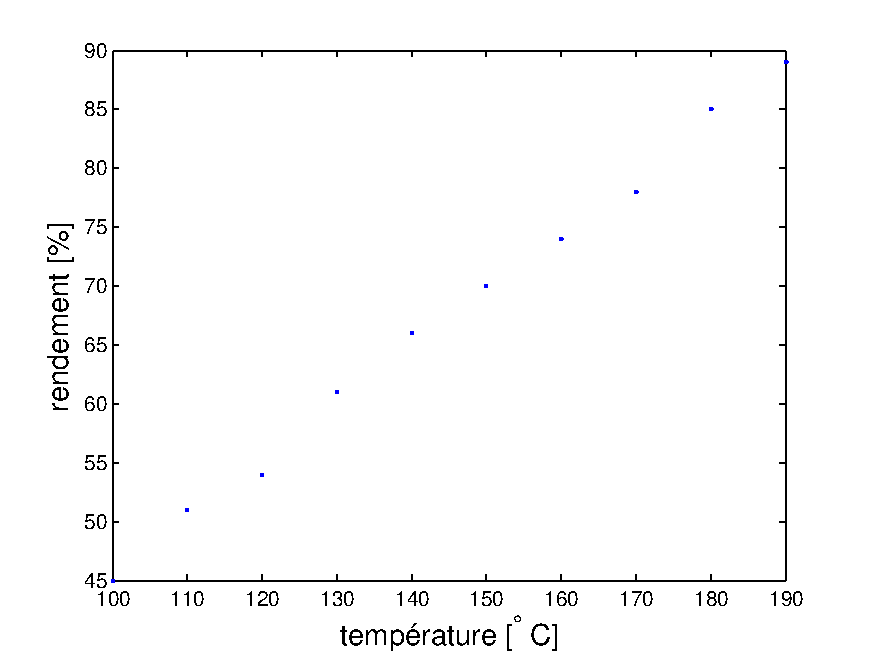
\includegraphics[scale=0.6]{4-Figures/2-scatter_plot_exp.pdf}
\caption{Diagramme de dispersion du rendement en fonction de la température}
\label{fig:scatter_plot_exp}
\end{figure}

On peut constater sur la figure \ref{fig:scatter_plot_exp} qu'il existe une relation forte entre le rendement et la température. Supposons que cette relation est linéaire, il est possible de modéliser ces données à l'aide de l'équation \eqref{eq:reg_lin_simple}. On calcule d'abord
\begin{align*}
 \sum_{i=1}^{10} x_i &=1450, &\hspace{1cm} & \overline{x}= \frac{1}{10} \sum_{i=1}^{10} x_i=145, & \sum_{i=1}^{10} x_i^2 = 218~500,\\
  \sum_{i=1}^{10} y_i&=673, &\hspace{1cm} & \overline{y}= \frac{1}{10} \sum_{i=1}^{10} y_i=67,3, & \sum_{i=1}^{10} Y_ix_i= 101~570.
\end{align*}
On obtient 
\begin{align*}
S_{xx}&=218~500-(1450)^2/10=8250, \cr
S_{xy}&=101~570-1450\times 673/10=3985.
\end{align*}
Et donc
\begin{align*}
\widehat{\beta_1} &= 3985/8250=0,483, \\
\widehat{\beta_0} &= 67,3-0,483\times145=-2,739.
\end{align*}
Le modèle de régression linéaire simple ajusté est $\widehat Y_i=-2,739+0,483x_i$. Ainsi, une augmentation de un degré Celsius de la température du procédé est associée à une augmentation moyenne de $0,483$ point de pourcentage du rendement du produit. Le modèle indique aussi qu'à une température nulle, le rendement attendu est de $-2,739\%$.

La figure~\ref{fig:reg_lin_exp} montre l'ajustement obtenu sous forme d'une droite. Dans ce cas-ci la relation linéaire semble très appropriée pour modéliser la relation entre les variables.

\begin{figure}[h!]
\centering
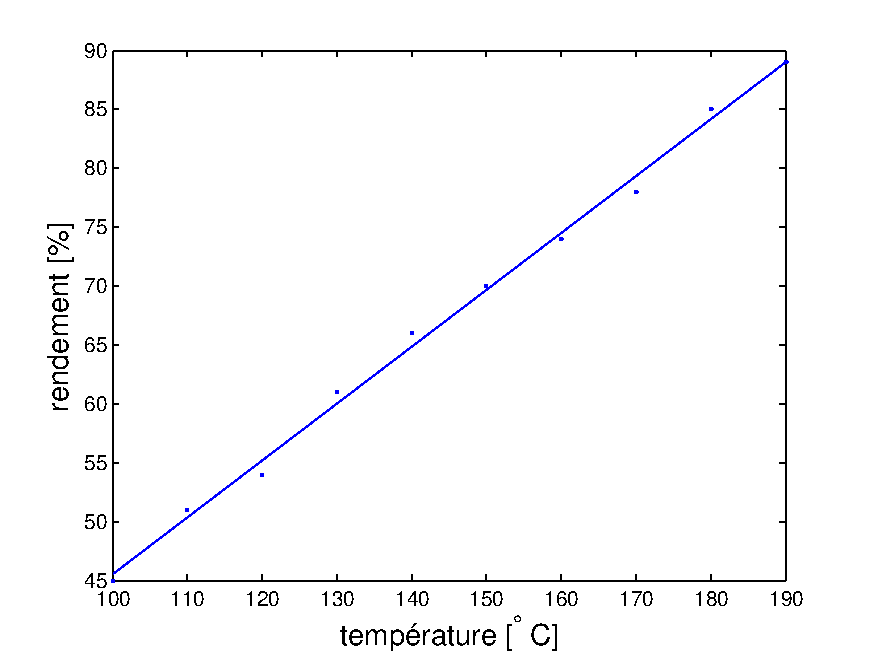
\includegraphics[scale=0.6]{4-Figures/2-reg_lin_exp.pdf}
\caption{Diagramme de dispersion du rendement en fonction de la température avec la droite de régression estimée superposée}
\label{fig:reg_lin_exp}
\end{figure}

On peut également estimer $\sigma^2$ à partir des données. Il faut d'abord calculer la valeur prédite et le résidu pour chacune des observations, comme au Tableau \ref{tab:cal_sigma2_exp}. L'équation~\eqref{sigma2} mène à
$$\widehat{\sigma}^2_{MV}=\frac{1}{10} \{(-0,561)^2+\cdots+(-0,0301)^2\}=\frac{7,224}{10}=0,7224.$$

\begin{table}[h!]
\caption{Tableau résumant $x_i$, $Y_i$, $\hat Y_i$ et $\widehat\varepsilon_i$, $i=1,\dots,10$ pour le calcul de $\widehat\sigma^2_{MV}$ dans l'exemple de la section \ref{exemple-RLS-interpretation}}
\label{tab:cal_sigma2_exp} \centering
\begin{tabular}{c|cccc}
$i$ & $x_i$& $Y_i$ & $\hat Y_i$ & $\widehat\varepsilon_i$ \\ \hline
1 & 100 & 45 & 45,561 &  -0,561 \\
2 & 110  & 51  & 50,391 & 0,609 \\
3 &  120 & 54  & 55,221 & -1,221 \\
4 & 130  & 61 & 60,051 & 0,949\\
5 & 140 & 66  & 64,881  &  1,119 \\
6 & 150  & 70 & 69,711  & 0,289\\
7 &160  & 74 & 74,541 & -0,541\\
8 & 170  & 78 & 79,371 & -1,371\\
9 & 180 & 85 & 84,201 & 0,799\\
10 & 190  & 89 & 89,031 & -0,031
\end{tabular}
\end{table}